%% Preamble
  \documentclass{homework}

  \hwTitle{M.O. 2} % Assignment title
  \hwDueDate{Sunday,\ July\ 28,\ 2013} % Due date
  \hwClass{Sargent RA} % Course/class
  \hwAuthor{Spencer Lyon} % Your name

  \usepackage[shortlabels]{enumitem}
  \usepackage{setspace}
  \usepackage{booktabs}

  \providecommand{\e}[1]{\ensuremath{\times 10^{#1}}}
  \usepackage{caption}

  % Set up listings
  \usepackage{listings}
  \usepackage{color}

  \definecolor{dkgreen}{rgb}{0,0.6,0}
  \definecolor{gray}{rgb}{0.5,0.5,0.5}
  \definecolor{mauve}{rgb}{0.58,0,0.82}

  \lstset{frame=tb,
    language=Python,
    aboveskip=3mm,
    belowskip=3mm,
    showstringspaces=false,
    columns=flexible,
    basicstyle={\small\ttfamily},
    numbers=left,
    stepnumber=5,
    numberstyle=\tiny\color{gray},
    keywordstyle=\color{blue},
    commentstyle=\color{dkgreen},
    stringstyle=\color{mauve},
    breaklines=true,
    breakatwhitespace=true
    tabsize=4
  }

%% New Commands I use alot
  % partial derivative as a fraction
  \newcommand{\fracpd}[2]{
    \ensuremath{\frac{\partial #1}{\partial #2}}
  }

  % fraction with parenthesis around it
  \newcommand{\pfrac}[2]{
    \ensuremath{ \left( \frac{#1}{#2} \right)}
  }

  % two row small bracketed matrix
  \newcommand{\sbmtwo}[2]{
   \ensuremath{ \left[\begin{smallmatrix} #1 \\ #2 \end{smallmatrix}\right]}
  }

  % two row bracketed matrix
  \newcommand{\bmtwo}[2]{
   \ensuremath{ \begin{bmatrix} #1 \\ #2 \end{bmatrix}}
  }

\begin{document}

\maketitle

\begin{homeworkProblem}[Problem 2.6]

  Consider the stochastic process $\{c_t,z_t\}$ defined by equations (1) in exercise 2.5. Assume the parameter values described in part b, item i. If possible, assume the initial conditions are such that $\{c_t,z_t\}$ is covariance stationary.

  \begin{enumerate}[a.]
    \item Compute the initial mean and covariance matrix that make the process covariance stationary.
    \item For the initial conditions in part a, compute numerical values of the following population linear regression: $$ c_{t+2} =\alpha_0  + \alpha_1 z_t + \alpha_2 z_{t-4} + w_t$$ where $\left[\begin{smallmatrix} 1 & z_t & z_{t-4} \end{smallmatrix}\right] = \left[\begin{smallmatrix} 0 & 0 & 0 \end{smallmatrix}\right]$
  \end{enumerate}

  \vspace{.2in}

  \problemAnswer{

    \begin{enumerate}[a.]
      \item As noted in my solution to problem 5, the system described there can be put in to the canonical form for a stochastic linear difference equation as follows:

        \begin{align*}
            &x_{t+1} = &A &x_t + &C &w_{t+1} \\
            &\left[\begin{matrix} c_{t+1} \\ c_{t} \\ z_{t+1} \\ z_{t} \\ 1 \end{matrix}\right] =
              &\begin{bmatrix}  % A
               \rho_1 & \rho_2 & \delta_1 & \delta_2 &  \alpha_c \\
               1 & 0 & 0 & 0 & 0 \\
               \gamma_1 & \gamma_2 & \phi_1 & \phi_2 & 0 \\
               0 & 0 & 1 & 0 & 0 \\
               0 & 0 & 0 & 0 & 1
               \end{bmatrix}
               &\left[\begin{matrix} c_t \\ c_{t-1} \\ z_t \\ z_{t-1} \\ 1 \end{matrix}\right] % x
               +
               &\begin{bmatrix} % C
               \psi_1 & 0 \\
               0 & 0 \\
              0 & \psi_2 \\
              0 & 0 \\
              0 & 0
              \end{bmatrix}
              &\begin{bmatrix} % w_{t+1}
                w_{1, t+1}\\
                w_{2, t+1}
              \end{bmatrix}
          \end{align*}

          Using this form, the covariance stationary mean is found by computing the eigenvector of A that corresponds to the single unit eigenvalue of A. I did this using the included python program and got that
          $$\mu = \begin{bmatrix}2 & 2 & 0 & 0 & 1\end{bmatrix}$$

          So solve for the covariance stationary covariance matrix, I simply used the command \texttt{doublej(A, C.dot(C.T))}. The matrix I got for $C_x$ is
          $$
          \begin{bmatrix}
            1.970 & 1.249 & 0.241 & 0.487 & 0.000\\
            1.249 & 1.970 & 0.071 & 0.241 & 0.000\\
            0.241 & 0.071 & 1.579 & 0.921 & 0.000\\
            0.487 & 0.241 & 0.921 & 1.579 & 0.000\\
            0.000 & 0.000 & 0.000 & 0.000 & 0.000\\
          \end{bmatrix}
          $$
      \item To solve for the coefficients in this problem I will use equation 2.5.3, which states $$\beta = (EYX') [E(XX')]^{-1}$$ where $X' = \left[\begin{smallmatrix} 1 & z_t & z_{t-4} \end{smallmatrix}\right]$ and $Y = c_{t+2}$. This allows me to write the following expression for $E(XX')$:
      $$
      E(XX') = E
      \begin{bmatrix}
      1 & z_t & z_{t-4} \\
      z_t & z_t^2 & z_{t-4} z_t \\
      z_{t-4} & z_{t-4} z_t & z_{t-4}^2 \\
      \end{bmatrix}
      $$

      I can now evaluate what these expressions are by passing the expectation through and noting from part a that $E[z_t] =0 \forall t$. This allows me to compute directly the first row and column of the matrix. To compute the rest of it I turn to the definition of covariance: $\text{cov}(x, y) = E(x - \mu_x) E(y - \mu_y)'$. Applying this definition and recalling that $\mu_z= 0$, I can simplify the matrix above in the following manner:

      $$
      E(XX') = E
      \begin{bmatrix}
      1 & z_t & z_{t-4} \\
      z_t & z_t^2 & z_{t-4} z_t \\
      z_{t-4} & z_{t-4} z_t & z_{t-4}^2 \\
      \end{bmatrix}
      =
      \begin{bmatrix}
      1 & 0 & 0 \\
      0 & \text{var}(z_t) & \text{cov}(z_{t-4}, z_t) \\
      0 & \text{cov}(z_{t-4}, z_t) & \text{var}(z_{t-4}) \\
      \end{bmatrix}
      $$

      The expressions above can be found in certain entries of $C_x(j)$:

      \begin{itemize}
        \item $\text{var}(z_t)$ is the 3, 3 entry of $C_x(0)$
        \item $\text{cov}(z_{t-4}, z_t)$ is the 3, 3 entry of $C_x(-4) = \left[A^4 C_x(0)\right]'$
        \item $\text{var}(z_t)$ is the 3, 3 entry of $C_x(0)$
        \item $\text{var}(z_{t-4})$ is also the 3, 3 entry of $C_x(0)$ because the distribution is time-invariant (covariance stationary)
      \end{itemize}

      Now to evaluate the other expectation.
      $$
      E(YX') = E
      \begin{bmatrix}
       c_{t+2} \\
       c_{t+2} z_t' \\
       c_{t+2} z_{t-4}' \\
      \end{bmatrix}
      $$

      The first row of this vector is easy and obvious. The other two rows can be computed directly by expanding out the definition of the covariance. I will only show this for the second row, but the third follows similarly.

      \begin{align*}
        \text{cov}(c_{t+2}, z_t)  &= E(c_{t+2} - \mu_c) E(z_t - \mu_z)' \\
          &= E(c_{t+2} z_t') + E(c_{t+2}(-\mu_z)') + E((-\mu_c) z_t') + E((-\mu_c) (-\mu_z)') \\
          &= E(c_{t+2} z_t') + E(c_{t+2})(-0)' + E((2) 0') + E((2) (0)') \\
          &= E(c_{t+2} z_t')
      \end{align*}

      which is the expression in the second row of $E(YX')$. This means that we can say the following two things:

      \begin{itemize}
         \item $E(c_{t+2} z_t') = \text{cov}(c_{t+2}, z_t)$, which is the $1, 3$ element of $C_x(2)$
         \item $E(c_{t+2} z_{t-4}') = \text{cov}(c_{t+2}, z_{t-4})$, which is the $1, 4$ element of $C_x(5)$
       \end{itemize}

      I am now finally ready to evaluate the expressions in each matrix, take the product of them, and obtain an expression for $\beta$.

      \begin{align*}
        \beta &= (EYX') [E(XX')]^{-1} \\
          &=
          \begin{bmatrix}
            2.000\\
            0.502\\
            -0.050\\
          \end{bmatrix}
          \begin{bmatrix}
            1.000 & 0.000 & 0.000\\
            0.000 & 1.579 & -0.034\\
            0.000 & -0.034 & 1.579\\
          \end{bmatrix}^{-1} \\
          &=
          \begin{bmatrix}
            2.000\\
            0.317\\
            -0.025\\
          \end{bmatrix}
      \end{align*}
    \end{enumerate}

    \setstretch{0.68}
    \lstinputlisting[language=Python, linerange={1-7, 14-73, 413-414, 495-571}]{../RMT4_Ch2.py}
    \setstretch{1.5}
    \qed
  }
\end{homeworkProblem}

\begin{homeworkProblem}[Problem 2.10]

  Let $P$ be a transition matrix for a Markov chain. Suppose that $P'$ has two distinct eigenvectors $\pi_1 , \pi_2$ corresponding to unit eigenvalues of $P'$ . Scale $\pi_1$ and $\pi_2$ so that they are vectors of probabilities (i.e., elements are nonnegative and sum to unity). Prove for any $\alpha \in [0, 1]$ that $\alpha \pi_1 + (1 - \alpha) \pi_2$ is an invariant function of P .

  \vspace{.2in}

  \problemAnswer{

    I am given that $\pi_1$ and $\pi_2$ are the only eigenvectors corresponding to the unit eigenvalues of $P$. Any convex combination of eigenvectors corresponding to the same eigenvalue is also an eigenvector corresponding to that same eigenvector. The quantity given in the problem ($\alpha \pi_1 + (1 - \alpha) \pi_2$) is a convex combination, which means that it is also an eigenvector corresponding to a unit eigenvalue of $P$. \medskip

    By definition, the eigenvectors of a Markov transition matrix $P$ corresponding to unit eigenvalues are invariant functions of $P$.  \qed

  }
\end{homeworkProblem}

\begin{homeworkProblem}[Problem 2.14]

  Consider a Markov chain with transition matrix
  $$
  \begin{bmatrix}
    .5 & .5 & 0 & 0 \\
    .1 & .9 & 0 & 0 \\
    0 & 0 & .9 & .1 \\
    0 & 0 & 0 & 1
  \end{bmatrix}
  $$
  with state space $X = \{e_i, i = 1, \dots, 4 \}$ where $e_i$ is the $i$th unit vector. A random variable $y_t$ is a function $y_t = \left[\begin{smallmatrix} 1 & 2 & 3 & 4  \end{smallmatrix}\right] x_t$ of the underlying state.

  \begin{enumerate}[a.]
    \item Find all stationary distributions of the Markov chain.
    \item Can you find a stationary distribution for which the Markov chain ergodic?
    \item Compute all possible limiting values of the sample mean $\frac{1}{T} \sum_{t=0}^{T-1} y_t$ as $T \rightarrow \infty$
  \end{enumerate}

  \vspace{.2in}

  \problemAnswer{

    \begin{enumerate}[a.]
      \item The stationary distributions of the matrix $P$ are the left eigenvectors associated with unit eigenvalues. Doing this computation for the given transition matrix yields the following stationary distributions:

      $$\pi_1 = \begin{bmatrix} 1/6 & 5/6 & 0 & 0\\ \end{bmatrix} $$
      $$ \pi_2 = \begin{bmatrix} 0 & 0 & 0 & 1\\  \end{bmatrix} $$

      Any convex combination of $\pi_1$ and $\pi_2$ is also a stationary distribution of $P$.

      \item To answer this question, I first need to find the invariant functions associated with the chain $P$. These are the right eigenvectors of $P$ and I found them to be:

        $$\bar{y}_1 = \begin{bmatrix} .5 & .5 & 0 & 0\end{bmatrix}$$
        $$ \bar{y}_2 =\begin{bmatrix} 0 & 0 & .5 & .5\end{bmatrix}$$

        Note that eigenvectors are only constant up to a scalar multiple, so it is fair to write them in terms of a scalar multiple, like so (Note that $\alpha$ and $\beta$ can be any real number):

        $$\bar{y}_1 = \begin{bmatrix} \alpha & \alpha & 0 & 0\end{bmatrix}$$
        $$ \bar{y}_2 =\begin{bmatrix} 0 & 0 & \beta & \beta\end{bmatrix}$$

        Now, any convex combination of the eigenvectors of a matrix is also an eigenvector of the same matrix. That means we have a continuum of stationary distributions of the form:

        \begin{align*}
           \gamma \pi_1 &+ (1 - \gamma) \pi_2 \\
           \gamma  \begin{bmatrix} 1/6 & 5/6 & 0 & 0\\ \end{bmatrix} &+ (1 - \gamma) \begin{bmatrix} 0 & 0 & 0 & 1\\ \end{bmatrix} \\
        \end{align*}

        where $\gamma \in [0, 1]$. There are 3 cases that we will examine separately:

        \begin{enumerate}[1.]
          \item $\gamma \in (0, 1)$: In this situation, there is positive probability on elements $1, 2$, and $4$ of the stationary distribution. This means that for the chain to be ergodic under these circumstances, elements $1, 2$, and $4$ of the invariant functions must be equal. We see that they are not. Therefore the chain is not ergodic when $\gamma \in (0, 1)$.
          \item $\gamma = 0$: Here the stationary distribution is $\pi_1$ and there is positive probability in elements $1$ and $2$. We also see that the invariant functions all have equal values for elements $1$ and $2$, therefore the chain is ergodic under $\pi_1$.
          \item $\gamma = 1$: This time the stationary distribution is $\pi_1$ and there is positive probability only in element $4$. All invariant functions have a constant scalar in as the 4th element, so the chain is also ergodic under $\pi_2$.
        \end{enumerate}

      \item The value of the sample mean will depend on the initial distribution $\pi_0$. However, regardless of the initial distribution, $\pi_t$ will eventually converge to one of the ergodic distributions and the sample mean will converge to the value implied by the ergodic distribution. In part b I showed that the only two ergodic distributions were $\pi_1$ and $\pi_2$. This means that the limiting values of the sample mean are simply the average of $\bar{y}$ weighted by the elements in $\pi_1$ and $\pi_2$. Those values are below.
      \begin{itemize}
        \item Under $\pi_1$: 1.83334
        \item Under $\pi_2$: 4.0
      \end{itemize}
    \end{enumerate}

    \setstretch{0.68}
    \lstinputlisting[language=Python, linerange={1-7, 14-15, 74-124, 572-622}]{../RMT4_Ch2.py}
    \setstretch{1.5}

    \qed

  }
\end{homeworkProblem}

\begin{homeworkProblem}[Problem 2.17 -- Lake model]

  A worker can be in one of two states, state 1 (unemployed) or state 2 (employed). At the beginning of each period, a previously unemployed worker has probability $\lambda = \int_{\bar{w}}^B dF(w)$ of becoming employed. Here $\bar{w}$ is his reservation wage and $F (w)$ is the c.d.f. of a wage offer distribution. We assume that $F(0) = 0,F(B) = 1$. At the beginning of each period an unemployed worker draws one and only one wage offer from $F$. Successive draws from $F$ are i.i.d. The worker's decision rule is to accept the job if $w \ge \bar{w}$ , and otherwise to reject it and remain unemployed one more period. Assume that $\bar{w}$ is such that $\lambda \in (0,1)$. At the beginning of each period, a previously employed worker is fired with probability $\delta \in (0,1)$. Newly fired workers must remain unemployed for one period before drawing a new wage offer.

  \begin{enumerate}[a.]
    \item Let the state space be $X = \{e_i, i=1, 2\}$, where $e_i$ is the $i$th unit vector. Describe the Markov chain on $X$ that is induced by the description above. Compute all stationary distributions of the chain. Under what stationary distributions, if any, is the chain ergodic?
    \item Suppose that $\lambda = .05, \delta = .25$ . Compute a stationary distribution. Compute the fraction of his life that an infinitely lived worker would spend unemployed.
    \item Drawing the initial state from the stationary distribution, compute the joint distribution $g_{ij} = \text{Prob}(x_t=e_i, x_{t-1}=e_j)$ for $i=1, 2, j=1, 2$.
    \item Define an indicator function by letting $I_{ij, t} = 1$ if $x_t = e_i, x_{t-1} = e_j$ at time $t$ and $0$ otherwise. Compute $$\lim_{t \rightarrow \infty} \frac{1}{T} \sum_{t=1}^T I_{ij, t}$$ for all four $i, j$ combinations.
    \item Building on your results in part d, construct method of moments estimators of $\lambda$ and $\delta$. Assuming that you know the wage offer distribution $F$, construct a method of moments estimator of the reservation wage $\bar{w}$.
    \item Compute maximum likelihood estimators of $\lambda$ and $\delta$.
    \item Compare the estimators you derived in parts e and f.
    \item \textit{Extra Credit.} Compute the asymptotic covariance matrix of the maximum likelihood estimators of $\lambda$ and $\delta$.
  \end{enumerate}

  \vspace{.2in}

  \problemAnswer{

    \begin{enumerate}[a.]
      % part a
      \item The state space can be represented by the transition matrix:
        $$ P =
        \begin{bmatrix}
          1- \lambda & \lambda \\
          \delta & 1 - \delta
        \end{bmatrix}
        $$

        The stationary distributions of this matrix are the left eigenvectors corresponding to the unit eigenvalues. In this case the eigenvalues are equal to $\psi_1 = 1, \psi_2 = 1 - \delta - \lambda$. The left eigenvector corresponding to the unit eigenvalue is given as (note I normalize so it sums to 1):
        $$\pi_0 =
        \begin{bmatrix}
          1 \\
          \delta / \lambda
        \end{bmatrix}
        \rightarrow
        \begin{bmatrix}
          \frac{\lambda }{\delta +\lambda} \\
          \frac{\delta }{\delta +\lambda }
        \end{bmatrix}
        $$

        To determine the ergodicity of this stationary distribution, I need to evaluate the invariant functions of the Markov chain. The invariant functions are the right eigenvectors corresponding to the unit eigenvalues. As noted above, there is a single unit eigenvalue for this process and it has a corresponding right eigenvector equal to
        $$ \xi =
        \begin{bmatrix}
          \alpha \\
          \alpha
        \end{bmatrix}
        $$

        This chain is ergodic because both elements of $\pi_0$ are positive and both elements of $\xi$ are equal.

      % part b
      \item When $\lambda=0.05$ and $\delta = 0.25$ the stationary distribution is $$ \pi_0 = \begin{bmatrix} 5/6 \\ 1/6 \end{bmatrix} $$ This means that the infinitely lived worker would expect to be un-employed for $5/6 \approx 83.33\%$ of his life.

      % part c
      \item In this problem, the values of $g_{ij}$ are given by equation 2.3.1, which in this case means
        $$g_{ij} = \text{Prob}(x_t=e_i, x_{t-1}=e_j) = \text{Prob}\left(x_t = e_i | x_{t-1} = e_j \right) \text{Prob}\left(x_{t-1} = e_j \right)$$ In this case $\text{Prob}\left(x_t = e_i | x_{t-1} = e_j \right)$ is simply the $ji$ element of $P$ and $\text{Prob}\left(x_{t-1} = e_j \right)$ is the $j$ element of $\pi_0$. Doing the computation yields
        \begin{itemize}
          \item $g_{11} = P_{11} \pi_{0, 1} = (1 - \lambda) \pi_{0, 1} = \frac{19}{20} \frac{5}{6} = \frac{19}{24}$
          \item $g_{12} = P_{21} \pi_{0, 1} = (\delta) \pi_{0, 2} = \frac{1}{4} \frac{1}{6} = \frac{1}{24}$
          \item $g_{21} = P_{12} \pi_{0, 2} = (\lambda) \pi_{0, 1} = \frac{1}{20} \frac{5}{6} = \frac{1}{24}$
          \item $g_{22} = P_{22} \pi_{0, 2} = (1 - \delta) \pi_{0, 2} = \frac{3}{4} \frac{1}{6} = \frac{1}{8}$
        \end{itemize}

      % part d
      \item In this problem I was asked to find the average value of an indicator function. The way the indicator function was defined makes this average equal to the expected value of $I_{ij}$. The expected value of an indicator function for a particular state is simply the probability of being in the particular state. Thus, I can say
          $$\lim_{t \rightarrow \infty} \frac{1}{T} \sum_{t=1}^T I_{ij, t} = E\left[I_{ij}\right] =  P(ij) = g_{ij}$$
          where $g_{ij}$ are the values from part c. The answer is
          \begin{itemize}
            \item $I_{11} = g_{11} = (1 - \lambda) \pi_{0, 1} = \frac{19}{24}$
            \item $I_{12} = g_{12} = (\delta) \pi_{0, 2} =  \frac{1}{24}$
            \item $I_{21} = g_{21} = (\lambda) \pi_{0, 1} = \frac{1}{24}$
            \item $I_{22} = g_{22} = (1 - \delta) \pi_{0, 2} = \frac{1}{8}$
          \end{itemize}

      % part e
      \item Let $\hat{I}_{ij}$ be the sample mean corresponding to the theoretical means calculated in the previous part. I will construct a method of moments estimator for $\lambda$ by letting $\frac{\hat{I}_{11}}{\hat{I}_{12}}$ equal to the equivalent ratio from the above. This will allow me to write an expression for $\hat{\lambda}$ (the MOM estimator of $\lambda$) only in terms of the sample moments on $\hat{I}_{ij}$ as follows.

        \begin{align*}
          \frac{\hat{I}_{11}}{\hat{I}_{21}} &= \frac{\lim_{t \rightarrow \infty} \frac{1}{T} \sum_{t=1}^T I_{11, t}}{\lim_{t \rightarrow \infty} \frac{1}{T} \sum_{t=1}^T I_{21, t}} \\
            &= \frac{(1 - \hat{\lambda}) \pi_{0, 1}}{(\hat{\lambda}) \pi_{0, 1}} \\
            &= \frac{1 - \hat{\lambda}}{\hat{\lambda}} \\
            \hat{\lambda} &= \frac{1}{\frac{\hat{I}_{11}}{\hat{I}_{21}} + 1} = \frac{\hat{I}_{12}}{\hat{I}_{11}+\hat{I}_{12}}
        \end{align*}

        Repeating a similar process for $\delta$ gives the following:

        \begin{align*}
          \frac{\hat{I}_{22}}{\hat{I}_{12}} &= \frac{\lim_{t \rightarrow \infty} \frac{1}{T} \sum_{t=1}^T I_{22, t}}{\lim_{t \rightarrow \infty} \frac{1}{T} \sum_{t=1}^T I_{12, t}} \\
            &= \frac{(1 - \hat{\delta}) \pi_{0, 1}}{(\hat{\delta}) \pi_{0, 1}} \\
            &= \frac{1 - \hat{\delta}}{\hat{\delta}} \\
            \hat{\delta} &= \frac{1}{\frac{\hat{I}_{22}}{\hat{I}_{12}} + 1} = \frac{\hat{I}_{21}}{\hat{I}_{21}+\hat{I}_{22}}
        \end{align*}

        To find a method of moments estimator for $\bar{x}$ (call is $\hat{\bar{w}}$), I will return to the definition of $\lambda$ and replace it with $\hat{\lambda}$ as such

        $$ \hat{\lambda} = \int_{\bar{w}}^B d F(w)$$

        Evaluating the integral (keeping in mind that $F(B) = 1$), I can solve for an expression for $\hat{\bar{w}}$. Note that I define $F^{-1}$ to be the inverse of the given $F(w)$ in the sense that if $F(x) = y$ then $F^{-1}(y) = x$.

        \begin{align*}
          \hat{\lambda} &= \int_{\bar{w}}^B d F(w) \\
            \hat{\lambda} &= F(B) - F(\hat{\bar{w}}) \\
            \hat{\lambda} &= 1 - F(\hat{\bar{w}}) \\
            \hat{\bar{w}} &= F^{-1}(1 - \hat{\lambda})
        \end{align*}

      % part f
      \item To compute the maximum likelihood estimators of $\lambda$ and $\delta$, I begin with the likelihood function given in section 2.2.9:
        $$L = \pi_{0, i_0} \prod_i \prod_j P_{ij}^{n_{ij}}$$
        where $n_{ij}$ the number of times a transition from state $i$ to state $j$ occurs in a sample data set. To obtain maximum likelihood estimators I write the likelihood function in terms of the free parameters $\lambda$ and $\delta$ and choose those parameters so that the likelihood function is maximized. It is often easier to do this when working with the log-likilihood function, which is just the natural logarithm of the likelihood function. Because the logarithm is a monotonic transformation the $\lambda$ and $\delta$ that maximize the log-likelihood function will also maximize the likelihood function. The log-likelihood function is:

        $$l = \log(L) = \log(\pi_{0, i_0}) + \sum_i \sum_j n_{ij} \log(P_{ij}) $$

        Taking the derivative of this function with respect to both parameters yields:

        \begin{align*}
          \fracpd{l}{\lambda} &= \sum_i \sum_j n_{ij} \frac{\partial P_{ij} / \partial \lambda}{P_{ij}} \\
          \fracpd{l}{\delta} &= \sum_i \sum_j n_{ij} \frac{\partial P_{ij} / \partial \delta}{P_{ij}}
        \end{align*}

        In terms of this problem, with the transition matrix $P$ given from part a, these expressions are evaluated as follows:

        \begin{align*}
          \fracpd{l}{\lambda} &= \sum_i \sum_j n_{ij} \frac{\fracpd{P_{ij}}{\lambda}}{P_{ij}} \\
            &= n_{11} \pfrac{-1}{1 - \lambda} + n_{12} \pfrac{1}{\lambda}+ n_{21}(0) + n_{22}(0) \\
          \fracpd{l}{\delta} &= \sum_i \sum_j n_{ij} \frac{\fracpd{P_{ij}}{\delta}}{P_{ij}} \\
            &= n_{11} (0) + n_{12} (0) + n_{21} \pfrac{1}{\delta}+ n_{22} \pfrac{-1}{1 - \delta}
        \end{align*}

        Finally, to obtain the maximum likelihood parameter estimates, I set these two equations equal to zero and solve them for $\delta$ and $\lambda$. Doing so yields the following:
          $$\tilde{\lambda} = \frac{n_{12}}{n_{11}+n_{12}}$$
          $$\tilde{\delta} = \frac{n_{21}}{n_{21}+n_{22}}$$

      % part g
      \item The method of moments and maximum likelihood estimators for $\lambda$ and $\delta$ are actually equivalent. This can be understood by expanding the values $\hat{I}_{ij}$  in the method of expression for the method of moment estimators. To show how to do this, I will outline a numerical algorithm that could be used to estimate $\hat{I}_{ij}$.

        \begin{itemize}
          \item Setup:
            \begin{itemize}
              \item Obtain, via simulation or otherwise, a sample chain $\{x\}_{t=1}^T$ that comes from the transition matrix.
              \item Determine what value each state is given in the chain. Express this as a vector $V$.
            \end{itemize}
          \item To estimate $\hat{I}_{ij}$
            \begin{itemize}
              \item Start with \texttt{n=0}
              \item For \texttt{n $\in [1,  T)$}
                \begin{itemize}
                  \item Let \texttt{a = $x_{t-1}$} and \texttt{b = $x_t$}
                  \item If \texttt{b == $V_j$ and a == $V_i$}, then \texttt{n = n+1}
                \end{itemize}
              \item Compute \texttt{$\hat{I}_{ij} $ = n / (T - 1)}
             \end{itemize}
        \end{itemize}

        If we plug this expression into the method of moment estimators, we will see that they end up being equal to the maximum likelihood estimators.

        \begin{align*}
          \hat{\lambda} &= \frac{\hat{I}_{12}}{\hat{I}_{11}+\hat{I}_{12}}  \\
            &= \frac{n_{12} / (T - 1)}{n_{11} /  (T - 1) + n_{12}  / (T - 1)} \\
            &= \frac{n_{12}}{n_{11} + n_{12}} \\
            &= \tilde{\lambda}
        \end{align*}

        \begin{align*}
          \hat{\delta} &= \frac{\hat{I}_{21}}{\hat{I}_{21}+\hat{I}_{22}} \\
            &= \frac{n_{21} / (T - 1)}{n_{21} / (T - 1) + n_{22} / (T - 1)} \\
            &= \frac{n_{21}}{n_{21} + n_{22}} \\
            &= \tilde{\delta}
        \end{align*}
        \qed
    \end{enumerate}

  }
\end{homeworkProblem}

\begin{homeworkProblem}[Problem 2.20 -- Random Walk]

  A scalar process $x_t$ follows the process
  $$ x_{t+1} = x_t + w_{t+1} $$
  where $w$ is an iid $N(0, 1)$ scalar process and $X_0 \sim N(\hat{x}_0, \Sigma_0)$. Each period, an observer receives two signals in the form of a $2 x 1$ vector $y_t$ that obeys
  $$ y_t = \left[\begin{smallmatrix} 1 \\ 1 \end{smallmatrix}\right] x_t + v_t $$
  where the $2 x 1$ process $v$ is iid with distribution $v_t \sim N(0, R)$ where $R = I = \left[\begin{smallmatrix} 1 & 0 \\ 0 & 1 \end{smallmatrix}\right]$.

  \begin{enumerate}[a.]
    \item Suppose that $\Sigma_0 = 1.36602540378444$. For $t \ge 0$, find formulas for $E[x_t|y_{t-1}]$, where $y_{t-1}$ is the history of $y_s$ for $s$ from $0$ to $t - 1$.
    \item Verify numerically that the matrix $A - KG$ in formula (2.9.3) is stable.
    \item Find an infinite-order vector autoregression for $y_t$ .
  \end{enumerate}

  \vspace{.2in}

  \problemAnswer{

    NOTE: I would like to acknowledge that Chase Coleman helped a great deal with this problem. \medskip

    This problem is set up similar as a system similar to the Kalman filter system defined by equations 2.7.1 and 2.7.2 with $A_0 = C = 1, R = I_{2x2}$, and $G= \left[\begin{smallmatrix} 1 \\ 1 \end{smallmatrix}\right]$, where $I$ is the identity matrix.

    \begin{enumerate}[a.]
      \item To begin, I would like to make one definition: $\hat{x}_t  = E \left[ x_t |y_{t-1} \right]$. With this in mind, I turn to the Kalman filter equations found in 2.7.12. Below I list those 4 equations, make substitutions for this problem, and present a simplified form of each equation:

        \begin{align*}
         a_t  &= y_t - G \hat{x}_t \\
          &= y_t - \bmtwo{1}{1} \hat{x}_t \\
          &= \begin{bmatrix} y - \hat{x}_t \\ y - \hat{x}_t \end{bmatrix}
        \end{align*}

        \begin{align*}
          K_t &= A_0 \Sigma_t G'(G \Sigma_t G' + R)^{-1} \\
          &= 1 \Sigma_t \bmtwo{1}{1}' \left(\bmtwo{1}{1} \Sigma_t \bmtwo{1}{1}' + \bmtwo{1 & 0}{0 & 1} \right)^{-1} \\
          &= \begin{bmatrix} \frac{\Sigma_t }{2 \Sigma_t +1} & \frac{\Sigma_t }{2 \Sigma_t +1} \end{bmatrix}
        \end{align*}

        \begin{align*}
          \hat{x}_{t+1} &= A_0 \hat{x}_t + K_t a_t\\
            &= 1 \hat{x}_t + \begin{bmatrix} \frac{\Sigma_t }{2 \Sigma_t +1} & \frac{\Sigma_t }{2 \Sigma_t +1} \end{bmatrix} \begin{bmatrix} y - \hat{x}_t \\ y - \hat{x}_t \end{bmatrix} \\
            &= \frac{\hat{x}_t + 2 y_t \Sigma_t }{2 \Sigma_t +1}
        \end{align*}

        \begin{align*}
          \Sigma_{t+1} &= CC' + K_tRK_t' + (A_0 - K_tG) \Sigma_t (A_0 K_t G)' \\
            &= 1 + K_t \bmtwo{1&0}{0&1} K_t' + \left( 1 - K_t \bmtwo{1}{1} \right) \Sigma_t \left( 1 - K_t \bmtwo{1}{1} \right)' \\
            &= \frac{3 \Sigma_t +1}{2 \Sigma_t +1}
        \end{align*}

        Together these 4 equations specify the value of $\hat{x}_t$.
      \item The value of $A - KG$, for this problem, is
        \begin{align*}
          A - KG &= 1 - \begin{bmatrix} \frac{\Sigma_t }{2 \Sigma_t +1} & \frac{\Sigma_t }{2 \Sigma_t +1} \end{bmatrix} \bmtwo{1}{1} \\
           & = \frac{1}{2 \Sigma_t + 1}
        \end{align*}

        I used an included python program so simulate the path of $\Sigma_t$, starting at $\Sigma_0 = 1.36602540378444$. Using this simulated path, I simulated the path of $A - KG$ and plotted it. I have included this path in Figure ~\ref{fig:p2_20b} and it is easy to see that the path is just constant, and therefore stable.

      \item To find an infinite order or time-invariant VAR expression for $y_t$, I turn to section equation 2.9.3 from section 2.9.2 in RMT4. This equation is

        $$y_t = G \sum_{j=0}^{\infty} (A - KG)^j K_{y_{t - j - 1}} + a_t $$

        Where
        \begin{itemize}
          \item $G = \sbmtwo{1}{1}$
          \item $(A -KG) = \frac{1}{2 \Sigma_t + 1}$
          \item $K_t = \begin{bmatrix} \frac{\Sigma_t }{2 \Sigma_t +1} & \frac{\Sigma_t }{2 \Sigma_t +1} \end{bmatrix}$
          \item $a_t = y_t - G \hat{x}_t$
        \end{itemize}
    \end{enumerate}
    \setstretch{0.68}
    \lstinputlisting[language=Python, linerange={1-7, 639-660}]{../RMT4_Ch2.py}
    \setstretch{1.5}
    \qed

  }
      \begin{figure}[!h]
        \centering
        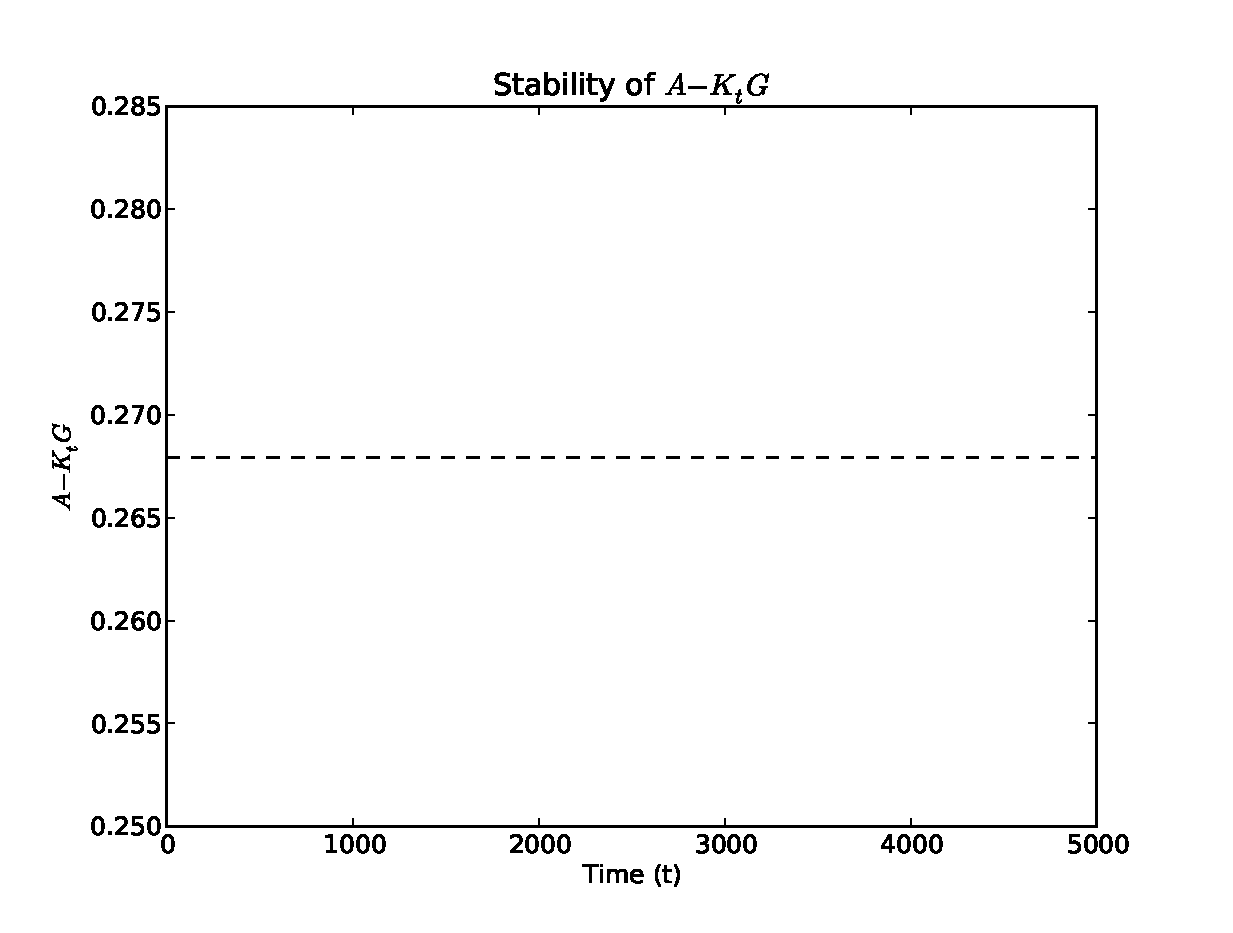
\includegraphics[width=5.5in]{./p2_20b.eps}
        \captionsetup{width=4in}
        \caption{\small Path of $A - KG$ for random walk process starting with $\Sigma_0 = 1.36602540378444$}
        \label{fig:p2_20b}
      \end{figure}
\end{homeworkProblem}

\begin{homeworkProblem}[Problem 2.24]

  A pair of scalar stochastic processes $(z_t, y_t)$ evolves according to the state system for $t \ge 0$:

  \begin{align*}
    z_{t+1} &= 0.9 z_t + w_{t+1} \\
    y_t &= z_t + v_t
  \end{align*}

  where $w_{t+1}$ and $v_t$ are mutually uncorrelated scalar Gaussian random variables with means of $0$ and variances of $1$. Furthermore, $Ew_{t+1}v_s = 0$ for all $t,s$ pairs. In addition, $z_0 \sim N(\hat{z}_0,\
  \Sigma_0).$

  \begin{enumerate}[a.]
    \item Is $\{z_t\}$ Markov? Explain
    \item Is $\{y_t\}$ Markov? Explain
    \item Define what it would mean for the scalar process $\{z_t\}$ to be \textit{covariance stationary}.
    \item Find values of $(\hat{z}_0, \Sigma_0)$ that make the process for $\{z_t\}$ covariance stationary.
    \item Assume that $y_t$ is observable, but that $z_t$ is not. Define what it would mean for the scalar process $y_t$ to be \textit{covariance stationary}.
    \item Describe in as much detail as you can how to represent the distribution of $y_t$ conditional on the infinite history $y_{t-1}$ in the form $y_t \sim N(E[y_t|y_{t-1}],\Omega_t)$.
  \end{enumerate}

  \vspace{.2in}

  \problemAnswer{

    \begin{enumerate}[a.]
      %part a
      \item Yes, $\{z_t\}$ is Markov because it satisfies the property that Prob$(z_t|z_{t-1} \dots z_{t-k}) = \text{Prob}(z_t|z_{t-1})$.

      % Part b
      \item I believe that $y_t$ is also Markov. I look at the expected value of $x$ and $y$ to argue my case.
        $$E[y_t] = E[z_t + v_t] = E [0.9z_{t-1} + w_{t+1}]  + 0 = 0.9 z_{t-1}$$

        $$ E[z_t] = E [0.9z_{t-1} + w_{t+1}] = 0.9 z_{t-1} + 0$$

        Therefore, I can say that $E[y_t] = E[z_t]$ and I have already explained how $z_t$ is Markov.

      % part c
      \item $z_t$ being covariance stationary would mean two things:
        \begin{enumerate}[1.]
          \item The expected value of $z_t$ is not a function of $t$. In other words $$E[z_t] = E[z_0] = \mu_z $$
          \item The sequence of auto-covariance matrices $E \left( z_{t+j} - E z_{t+j} \right) \left( z_t - E z_t \right) '$ depend only on the separation dates $j$ and not the time period $t$.
        \end{enumerate}

      % part d
      \item To find the values of $\hat{z}_0$ and $\Sigma_0$ are found using the equations in a table from section 2.4.2. I repeat the necessary formulas here. Note that $\hat{z}_0 = \mu$ and $C_x(0) = \Sigma_0$.
        $$(I - A_0) \mu = 0 \Longrightarrow (1 - 0.9) \hat{z}_0 = 0 \Longrightarrow \hat{z}_0 = 0$$
        $$C_x(0) = A_0C_x(0)A_0' + CC' \Longrightarrow \Sigma_0 = .9 \Sigma_0 .9 + 1 \Longrightarrow \Sigma_0 = 5.2632$$

      % part e
      \item If $y_t$ were covariance stationary, the same two properties discussed in part c. would apply. However, these properties would have deeper implications. I will discuss them one at a time.
        \begin{enumerate}[1.]
          \item The expected value of $y_t$ is not a function of $t$. In part b. I explained how $E[y_t] = E[z_t]$. So for property 1 to hold for $y_t$, it would also hold for $z_t$.
          \item The sequence of auto-covariance matrices $E \left( y_{t+j} - E y_{t+j} \right) \left( y_t - E y_t \right) '$ depend only on the separation dates $j$ and not the time period $t$. I will work directly with the expression for the auto-covariance matrix, do some algebra, substitute $y_t = z_t + v_t$, and do some more algebra below. Note that I use the property that $y_t$ has a time-independent mean going from line 1 to line 2 below.
            \begin{align*}
              &E \left( y_{t+j} - E y_{t+j} \right) \left( y_t - E y_t \right) ' \\
              &E(y_{t+j}y_t) - \mu_y^2 \\
              &E([z_{t+j} + v_{t+j}][z_t + v_t]) - \mu_z^2 \\
              &E[z_{t+j}z_t] + E[z_{t+j}v_t] + E[v_{t+j}z_t] + E[v_{t+j}v_t] - \mu_z^2 \\
              &E[z_{t+j} z_t] + \text{cov}(z_{t+j}, v_t) + \text{cov}(v_{t+j}, z_t) + \text{cov}(z_{t+j}, v_t) - \mu_z^2 \\
              &E[z_{t+j} z_t] - \mu_z^2 \\
               &E\left( z_{t+j} - E z_{t+j} \right) \left( z_t - E z_t \right) '
            \end{align*}
        \end{enumerate}
         So \footnote{The last two steps in the above calculations were a bit tricky. I used the assumption that the mean of $z$ was time independent, and that may have not been permissible in this situation.}, if $y_t$ is covariance stationary, then the unobserved $z_t$ is also covariance stationary.

      % part f
      \item A very useful theorem from econometrics explains the distribution of the sum of normally distributed variables (Dr. Jim McDonald calls it the useful theorem, so I don't actually know its real name). Applying the useful theorem to this problem reveals that $$y_t \sim N \left(\mu_{z_t} + \mu_{v_t}, \Sigma_{z_t} + \Sigma_{v_t} - 2 \text{cov}(z_t, v_t) \right)$$ In this case we can simplify the expression for the variance because we know $z_t$ and $v_t$ are independent, so cov$(z_t, v_t) = 0$. We are given that $\Sigma_{v_t} = 1 \forall t$, which is constant across time. Therefore, the distribution of $y_t$ can be simplified as: $$y_t \sim N(\mu_{z_t}, \Sigma_{z_t} + 1)$$ This identifies the matrix $\Omega$ as $\Sigma_z + 1$. \medskip

      As in the model studied by Muth (described in section 2.8.1), the conditional expectation $E[y_t |y^{t-1}]$ can be given by equation 2.8.6b, which is
      $$ E[y_t |y^{t-1}] = G A^j \hat{x}_t$$
      Making the necessary substitutions for this problem we have
      $$E[y_t |y^{t-1}] =0.9^j \hat{x}_t $$
      \qed
    \end{enumerate}

  }
\end{homeworkProblem}

\end{document}

